% Method
\section{Method}
\label{sec:method}

Our system consists of two coupled components: (1) a rectified-flow GNN that maps each agent's local observation to a preferred velocity, and (2) CV-PIBT, which takes these preferred velocities as inputs and resolves inter-agent conflicts to produce collision-aware committed velocities. At each planning step, both components execute in sequence.

\subsection{Problem Formulation}

We consider $N$ agents in a 2D continuous workspace $\mathcal{W} \subset \mathbb{R}^2$. Agent $i$ has position $p_i \in \mathcal{W}$, body radius $r_a$, and goal $g_i \in \mathcal{W}$. At each discrete time step, the planner outputs a velocity $u_i \in \mathbb{R}^2$ for each agent subject to $\|u_i\|_\infty \leq v_{\max}$. Two agents $i$ and $j$ collide if $\|p_i - p_j\|_2 < 2r_a$ at any point during a step. An agent reaches its goal if $\|p_i - g_i\|_2 \leq r_a$. The objective is to maximize the fraction of agents that reach their goals within a fixed step budget, while minimizing cumulative pair-timestep collisions.

\subsection{Rectified-Flow GNN}
\label{sec:method:flow}

\subsubsection{Input Representation}

Each agent $i$ receives an egocentric local observation: a $(2k{+}1) \times (2k{+}1)$ map with three channels encoding local obstacles, positions of other agents (within the observation window), and the agent's own goal indicator. We use $k{=}5$, giving an $11 \times 11$ map. In addition, agent $i$ has a five-dimensional auxiliary feature vector $a_i = [\hat{d}_{i,x},\; \hat{d}_{i,y},\; \|g_i - p_i\|_2,\; (u_i)_x,\; (u_i)_y]$, where $\hat{d}_i = (g_i - p_i)/\|g_i - p_i\|_2$ is the unit direction to goal and $(u_i)_x, (u_i)_y$ is the agent's current velocity.

\subsubsection{CNN Visual Encoder}

The three-channel observation map is processed by a shared CNN:
\begin{align*}
  &\text{Conv}(3 \to 64, 3\!\times\!3) \to \text{BN} \to \text{SiLU} \to \text{MaxPool}(2), \\
  &\text{Conv}(64 \to 128, 3\!\times\!3) \to \text{BN} \to \text{SiLU} \to \text{MaxPool}(2), \\
  &\text{Conv}(128 \to 256, 3\!\times\!3) \to \text{BN} \to \text{SiLU} \to \text{Flatten}.
\end{align*}
The flattened CNN output is concatenated with the five auxiliary features and projected through a visual projection head:
\[
  h_i^{\text{vis}} = \text{SiLU}(\text{LayerNorm}(\text{Linear}(d_{\text{cnn}}+5,\; 1024))) \cdot (1 - m_d),
\]
where $m_d \sim \text{Bernoulli}(0.15)$ is dropout applied during training.

\subsubsection{Communication Graph}

Agents within communication radius $r_c$ are connected by an undirected edge in a dynamic graph $\mathcal{G}_t = (\mathcal{V}, \mathcal{E}_t)$ where $\mathcal{E}_t = \{(i,j) : \|p_i - p_j\|_2 \leq r_c\}$. We use $r_c = 6r_a$ in all experiments.

\subsubsection{Flow GNN Architecture}

At inference step $s$ of the rectified-flow integration (described below), agent $i$'s GNN input is:
\[
  z_i^{(0)} = [h_i^{\text{vis}};\; v_t^{(i)};\; t] \in \mathbb{R}^{1024 + 2 + 1},
\]
where $v_t^{(i)} \in \mathbb{R}^2$ is the current noisy flow variable and $t \in [0,1]$ is the flow time. This is projected to the GNN hidden dimension $d_h = 1024$ before message passing.

The GNN consists of $L=6$ GraphSAGE layers~\cite{hamilton2017graphsage}, each implemented as:
\[
  z_i^{(\ell+1)} = \text{SiLU}\left(\text{LayerNorm}\left(W_\ell \cdot \left[z_i^{(\ell)} \;\|\; \text{mean}_{j \in \mathcal{N}(i)} z_j^{(\ell)}\right] + z_i^{(\ell)}\right)\right),
\]
where $\|\cdot\|$ denotes concatenation and the residual connection $+z_i^{(\ell)}$ is applied after the norm and nonlinearity, projecting the sum back via a learned linear layer of width $d_h$.

\subsubsection{Output Heads}

The final GNN representation $z_i^{(L)}$ feeds three heads:
\begin{itemize}
  \item \textbf{Flow head}: $\hat{u}_i = \text{Linear}(512 \to 2)(\text{SiLU}(\text{Dropout}(\text{Linear}(1024 \to 512)(\text{SiLU}(\text{Dropout}(z_i^{(L)}))))))$. This outputs the predicted velocity field $f_\theta(v_t, t, h_i) \in \mathbb{R}^2$.
  \item \textbf{Action head}: a 5-class discrete action classifier trained with cross-entropy, used as an auxiliary training signal.
  \item \textbf{Wait-logit head}: a scalar $w_i$ with learnable scale $s_w$ and bias $b_w$; $\sigma(s_w \cdot w_i + b_w)$ is the probability that agent $i$ should wait. This is used as a soft prior during candidate scoring in CV-PIBT.
\end{itemize}

\subsubsection{Rectified Flow Training and Inference}

Training follows the rectified flow framework~\cite{liu2023rectifiedflow}. Given an expert velocity $x_1 = u_i^{\text{expert}}$ from an EECBS~\cite{li2021eecbs} demonstration and noise $x_0 \sim \mathcal{N}(0, I)$, we form the linear interpolant:
\[
  x_t = t \cdot x_1 + (1 - t) \cdot x_0, \quad t \sim \mathcal{U}[0,1].
\]
The target is the constant vector field $x_1 - x_0$, and the training loss is:
\[
  \mathcal{L}_{\text{flow}} = \mathbb{E}_{t, x_0, x_1}\bigl[\|f_\theta(x_t, t, h_i) - (x_1 - x_0)\|_2^2\bigr].
\]
Total training loss adds cross-entropy for the action head and binary cross-entropy for the wait head, each weighted at $0.1$.

At inference, we integrate $k=3$ Euler steps from $v_0 \sim \mathcal{N}(0, I)$:
\[
  v_{s+1} = v_s + \frac{1}{k} \cdot f_\theta\!\left(v_s,\; \frac{s}{k},\; h_i\right), \quad s = 0, 1, 2.
\]
The final $v_3$ is taken as the preferred velocity $\tilde{u}_i$ for agent $i$, clipped to $[-v_{\max}, v_{\max}]^2$.

\subsection{CV-PIBT}
\label{sec:method:shield}

CV-PIBT resolves velocity conflicts among the $N$ preferred velocities $\{\tilde{u}_i\}$ produced by the flow GNN. It generalizes the discrete PIBT algorithm~\cite{okumura2022pibt} to continuous space by operating on a set of scored candidate velocities rather than graph-adjacent positions.

\subsubsection{Candidate Velocity Set}

For each agent $i$, we construct a set $\mathcal{C}_i$ of $19$ candidate velocities:
\begin{enumerate}
  \item The preferred velocity $\tilde{u}_i$ (clipped to $v_{\max}$).
  \item The preferred velocity at half magnitude: $0.5 \cdot \tilde{u}_i$.
  \item Sixteen evenly-spaced directions at full speed $v_{\max}$: $v_{\max} \cdot [\cos(2\pi k/16),\; \sin(2\pi k/16)]$ for $k = 0, \ldots, 15$.
  \item The zero velocity (wait).
\end{enumerate}

\subsubsection{Candidate Scoring}

Each candidate $v \in \mathcal{C}_i$ receives an alignment score:
\[
  s(v) = \frac{v \cdot \hat{u}_i}{\|\hat{u}_i\|_2},
\]
where $\hat{u}_i = \tilde{u}_i / \|\tilde{u}_i\|_2$ is the unit preferred direction. Candidates are sorted in descending order of $s(v)$; the zero-velocity candidate is always placed last.

\subsubsection{Priority Ordering}

Agents are processed in descending order of a priority score. We use the remaining distance to goal $\|g_i - p_i\|_2$ as the default priority, with ties broken by agent index. Priorities are recomputed at each time step.

\subsubsection{Conflict Resolution with Backtracking}

Algorithm~\ref{alg:cvpibt} gives the full procedure. The key invariant is that once an agent $i$ commits a velocity $u_i^* \in \mathcal{C}_i$, that velocity is not subsequently changed unless a lower-priority agent fails to find a conflict-free candidate, triggering backtracking into agent $i$.

\begin{algorithm}[t]
\caption{CV-PIBT($\{\tilde{u}_i\}$, $\{p_i\}$, $\{g_i\}$, $r_a$, $\Delta t$)}
\label{alg:cvpibt}
\small
\SetAlgoLined
\KwIn{Preferred velocities $\{\tilde{u}_i\}$; positions $\{p_i\}$; goals $\{g_i\}$; agent radius $r_a$; time step $\Delta t$}
\KwOut{Committed velocities $\{u_i^*\}$}
$\text{committed} \leftarrow \{\}$\;
Sort agents by priority $\pi(i) = \|g_i - p_i\|_2$ descending\;
\For{each agent $i$ in priority order}{
  $u_i^* \leftarrow \textsc{Assign}(i,\; \mathcal{C}_i,\; \text{committed},\; \text{depth}=0)$\;
  $\text{committed}[i] \leftarrow u_i^*$\;
}
\Return{$\{u_i^*\}$}\;

\BlankLine
\SetKwFunction{FAssign}{Assign}
\SetKwProg{Fn}{Function}{:}{}
\Fn{\FAssign{$i$, $\mathcal{C}$, committed, depth}}{
  \ForEach{candidate $v \in \mathcal{C}_i$ sorted by $s(v)$ descending}{
    $p_i' \leftarrow p_i + v \cdot \Delta t$\;
    \lIf{$p_i'$ is inside an obstacle}{\textbf{continue}}
    $\text{ok} \leftarrow \texttt{True}$\;
    \ForEach{agent $j \in \text{committed}$}{
      \lIf{$\neg\textsc{SafePair}(p_i, v, p_j, u_j^*, r_a, \Delta t)$}{$\text{ok} \leftarrow \texttt{False}$; \textbf{break}}
    }
    \If{ok}{
      \Return{$v$}\;
    }
  }
  \tcc{No candidate found; attempt backtracking}
  \If{depth $<$ 3}{
    \ForEach{agent $j \in \text{committed}$ blocking $i$}{
      $\mathcal{C}_j' \leftarrow \mathcal{C}_j \setminus \{u_j^*\}$\;
      $u_j^{\text{new}} \leftarrow \textsc{Assign}(j,\; \mathcal{C}_j',\; \text{committed} \setminus \{j\},\; \text{depth}+1)$\;
      \If{$u_j^{\text{new}} \neq \varnothing$}{
        $\text{committed}[j] \leftarrow u_j^{\text{new}}$\;
        \Return{\FAssign{$i$, $\mathcal{C}_i$, committed, depth+1}}\;
      }
    }
  }
  \Return{$\mathbf{0}$}\tcc*{Fall back to wait}
}

\BlankLine
\SetKwFunction{FSafePair}{SafePair}
\Fn{\FSafePair{$p_i$, $v_i$, $p_j$, $v_j$, $r_a$, $\Delta t$}}{
  $p_i' \leftarrow p_i + v_i \Delta t$;\quad $p_j' \leftarrow p_j + v_j \Delta t$\;
  \lIf{$\|p_i' - p_j'\|_2 < 2r_a$}{\Return{\texttt{False}}}
  $\delta p \leftarrow p_i - p_j$;\quad $\delta v \leftarrow v_i - v_j$\;
  $t^* \leftarrow -(\delta p \cdot \delta v)/\|\delta v\|_2^2$ (clamped to $[0, \Delta t]$)\;
  $d^* \leftarrow \|\delta p + \delta v \cdot t^*\|_2$\;
  \lIf{$d^* < 2r_a$}{\Return{\texttt{False}}}
  \Return{\texttt{True}}\;
}
\end{algorithm}

\textbf{SafePair} checks two conditions for agents $i$ and $j$: (a) their next positions (after integrating for $\Delta t$) must be separated by at least $2r_a$, and (b) the minimum separation during the time interval $[0, \Delta t]$ (evaluated at the time of closest approach $t^*$) must also be at least $2r_a$.

\subsubsection{Fallback for Unassigned Agents}

In rare cases where the backtracking budget is exhausted, the agent commits the zero velocity. Agents that have not yet been processed in a given step (i.e., low-priority agents whose conflict resolution is deferred within a recursive call) fall back to the clipped preferred velocity from the flow GNN.

\subsection{System Integration}

At each planning step, the flow GNN takes $3$ Euler steps to produce preferred velocities (wall time $\approx 8$\,ms for $N{=}100$ on a single GPU). CV-PIBT then resolves conflicts in $O(N \cdot |\mathcal{C}| \cdot N_{\text{committed}})$ worst-case time per step. All agents then integrate their committed velocities for one step of duration $\Delta t = 1$.

Figure~\ref{fig:qualitative} shows example trajectories from the combined system in a random map.

\begin{figure}[t]
  \centering
  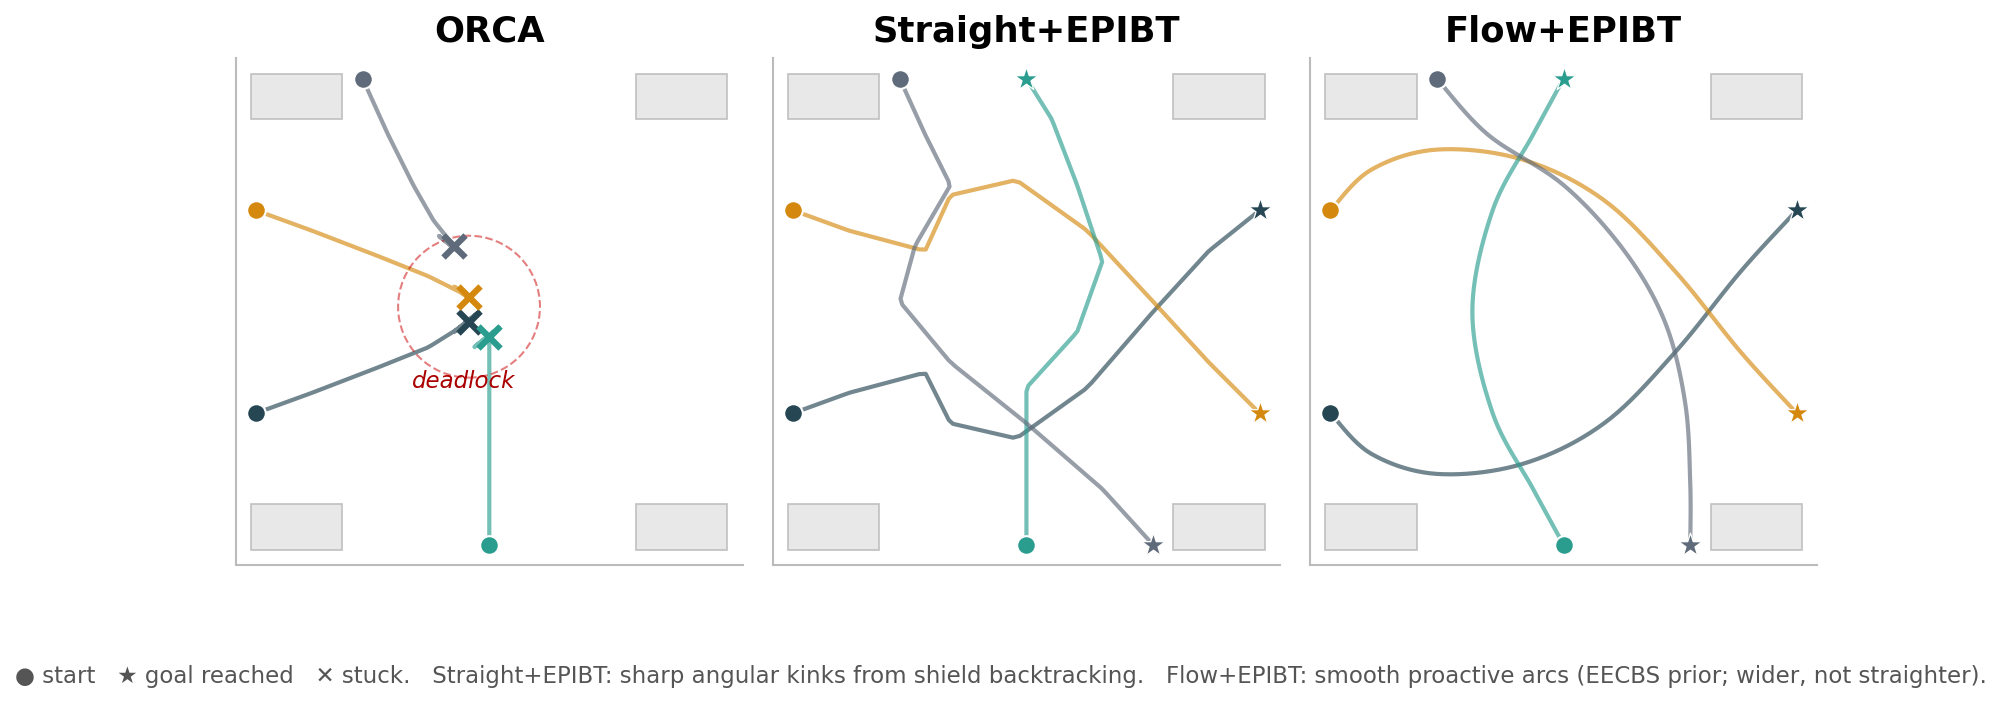
\includegraphics[width=\linewidth]{figures/fig5_qualitative_trajectories}
  \caption{Qualitative trajectory comparison on random-32-32-10 with $N{=}10$ agents over 512 steps. Each column shows a different conflict-resolution strategy with the same start/goal configuration. ORCA deadlocks at symmetric conflicts (crosses); Straight+CV-PIBT resolves deadlocks but takes angular detours; Flow+CV-PIBT produces smooth, proactive arcs that clear inter-agent conflicts earlier.}
  \label{fig:qualitative}
\end{figure}
